
%{{第二十八回}}{第二十八回}}

\chapter{蒋玉菡情赠茜香罗 薛宝钗羞笼红麝串}

{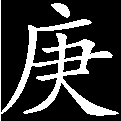
\includegraphics[width=3mm]{../Images/00004}\kaishu 茜香罗、红麝串写于一回,盖琪官虽系优人,后回与袭人供奉玉兄宝卿得同终始者,非泛泛之文也。}

{\kaishu 自``闻曲''回以后,回回写药方,是白描颦儿添病也。}

话说林黛玉只因昨夜晴雯不开门一事,错疑在宝玉身上。至次日,又可巧遇见饯花之期,正是一腔无明正未发泄,又勾起伤春愁思,因把些残花落瓣去掩埋,由不得感花伤己,哭了几声,便随口念了几句。不想宝玉在山坡上,听见是黛玉之声,先不过是点头感叹;次后听到``侬今葬花人笑痴,他年葬侬知是谁'',``一朝春尽红颜老,花落人亡两不知''等句,不觉恸倒山坡之上,怀里兜的落花撒了一地。试想林黛玉的花颜月貌,将来亦到无可寻觅之时,宁不心碎肠断!既黛玉终归无可寻觅之时,推之于他人,如宝钗、香菱、袭人等,亦可到无可寻觅之时矣。宝钗等终归无可寻觅之时,则自己又安在哉?且自身尚不知何在何往,则斯处、斯园、斯花、斯柳,又不知当属谁姓矣!{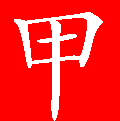
\includegraphics[width=3mm]{../Images/00002}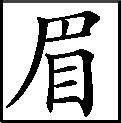
\includegraphics[width=3mm]{../Images/00010}\footnotesize \kaishu 不言炼句炼字,辞藻工拙,只想景、想情、想事、想理,反复推求,悲伤感慨,乃玉兄一生天性。真颦儿之知己,则实无再有者。昨阻余批《葬花吟》之客,嫡是玉兄之化身无疑。余几作点金成铁之人,笨甚笨甚!}\href{../Text/part0032_split_000.html\#lnkback_1_a}{\textsuperscript{①}}因此一而二,二而三,反复推求了去,{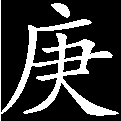
\includegraphics[width=3mm]{../Images/00004}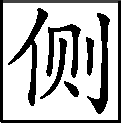
\includegraphics[width=3mm]{../Images/00011}\footnotesize \kaishu 百转千回矣。}真不知此时此际欲为何等蠢物,杳无所知,逃大造,出尘网,使可解释这段悲伤。{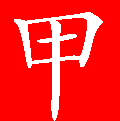
\includegraphics[width=3mm]{../Images/00002}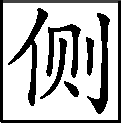
\includegraphics[width=3mm]{../Images/00011}\footnotesize \kaishu 非大善知识,说不出这句话来。}正是:

花影不离身左右,鸟声只在耳东西。{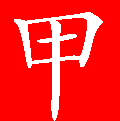
\includegraphics[width=3mm]{../Images/00002}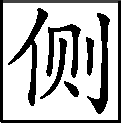
\includegraphics[width=3mm]{../Images/00011}\footnotesize \kaishu 二句作禅语参。}

{{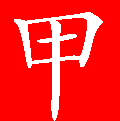
\includegraphics[width=3mm]{../Images/00002}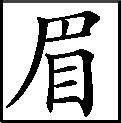
\includegraphics[width=3mm]{../Images/00010}\footnotesize \kaishu 一大篇《葬花吟》却如此收拾,真好机杼笔仗,令人焉得不叫绝称奇!}}

那黛玉正自悲伤,忽听山坡上也有悲声,心下想道:``人人都笑我有些痴病,难道还有一个痴子不成?''{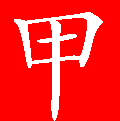
\includegraphics[width=3mm]{../Images/00002}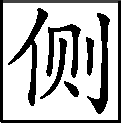
\includegraphics[width=3mm]{../Images/00011}\footnotesize \kaishu 岂敢岂敢。}想着,抬头一看,见是宝玉。林黛玉看见,便道:``啐!我当是谁,原来是这个狠心短命的\ldots{}\ldots{}''刚说到``短命''二字,又把口掩住,{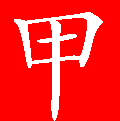
\includegraphics[width=3mm]{../Images/00002}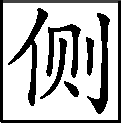
\includegraphics[width=3mm]{../Images/00011}\footnotesize \kaishu ``情情'',不忍道出``的''字来。 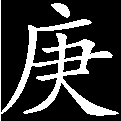
\includegraphics[width=3mm]{../Images/00004}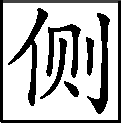
\includegraphics[width=3mm]{../Images/00011}\footnotesize \kaishu ``情情''。不忍也。}长叹了一声,自己抽身便走了。

这里宝玉悲恸了一回,见黛玉去了,便知黛玉看见他躲开了,自己也觉无味,抖抖土起来,下山寻归旧路,{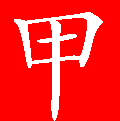
\includegraphics[width=3mm]{../Images/00002}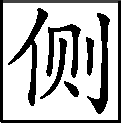
\includegraphics[width=3mm]{../Images/00011}\footnotesize \kaishu 折得好,誓不写开门见山文字。}往怡红院来。可巧{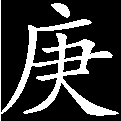
\includegraphics[width=3mm]{../Images/00004}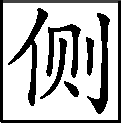
\includegraphics[width=3mm]{../Images/00011}\footnotesize \kaishu 哄人字眼。}看见林黛玉在前头走,连忙赶上去,说道:``你且站住。我知你不理我,我只说一句话,从今以后撂开手。''{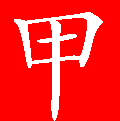
\includegraphics[width=3mm]{../Images/00002}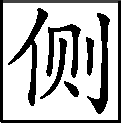
\includegraphics[width=3mm]{../Images/00011}\footnotesize \kaishu 非此三字难留莲步,玉兄之机变如此。}林黛玉回头见是宝玉,待要不理他,听他说``只说一句话,从此撂开手'',这话里有文章,少不得站住说道:``有一句话,请说来。''宝玉笑道:``两句话,说了你听不听?''{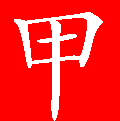
\includegraphics[width=3mm]{../Images/00002}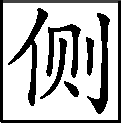
\includegraphics[width=3mm]{../Images/00011}\footnotesize \kaishu 相离尚远,用此句补空,好近阿颦。}黛玉听说,回头就走。{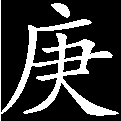
\includegraphics[width=3mm]{../Images/00004}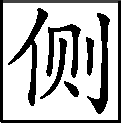
\includegraphics[width=3mm]{../Images/00011}\footnotesize \kaishu 走的是。}宝玉在身后面叹道:``既有今日,何必当初!''{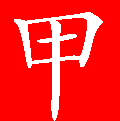
\includegraphics[width=3mm]{../Images/00002}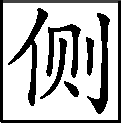
\includegraphics[width=3mm]{../Images/00011}\footnotesize \kaishu 自言自语,真是一句话。}林黛玉听见这话,由不得站住,回头道:``当初怎么样?今日怎么样?''宝玉叹道:{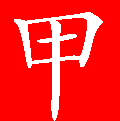
\includegraphics[width=3mm]{../Images/00002}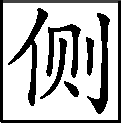
\includegraphics[width=3mm]{../Images/00011}\footnotesize \kaishu 以下乃答言,非一句话也。}``当初姑娘来了,那不是我陪着顽笑?{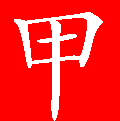
\includegraphics[width=3mm]{../Images/00002}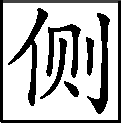
\includegraphics[width=3mm]{../Images/00011}\footnotesize \kaishu 我阿颦之恼,玉兄实摸{[}头{]}不着,不得不将自幼之苦心实事一诉,方可明心,以白今日之故,勿作闲文看。}凭我心爱的,姑娘要,就拿去;我爱吃的,听见姑娘也爱吃,连忙干干净净收着等姑娘吃。一桌子吃饭,一床上睡觉。丫头们想不到的,我怕姑娘生气,我替丫头们想的到。我心里想着:姊妹们从小儿长大,亲也罢,热也罢,和气到了头,才见得比人好。{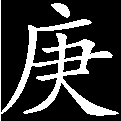
\includegraphics[width=3mm]{../Images/00004}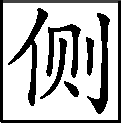
\includegraphics[width=3mm]{../Images/00011}\footnotesize \kaishu 要紧语。}如今谁承望姑娘人大心大,{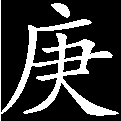
\includegraphics[width=3mm]{../Images/00004}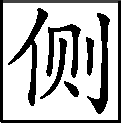
\includegraphics[width=3mm]{../Images/00011}\footnotesize \kaishu 反派不是。}不把我放在眼里,倒把外四路的什么宝姐姐{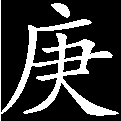
\includegraphics[width=3mm]{../Images/00004}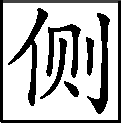
\includegraphics[width=3mm]{../Images/00011}\footnotesize \kaishu 心事。}凤姐姐{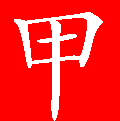
\includegraphics[width=3mm]{../Images/00002}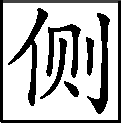
\includegraphics[width=3mm]{../Images/00011}\footnotesize \kaishu 用此人瞒看官也,瞒颦儿也。心动阿颦在此数句也。一节颇似说辞,玉兄口中却是衷肠话。}的放在心坎儿上,倒把我三日不理四日不见的。我又没个亲兄弟亲姊妹------虽然有两个,你难道不知道是和我隔母的?我也和你是独出,只怕同我的心一样。谁知我是白操了这个心,弄的我有冤无处诉!''{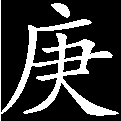
\includegraphics[width=3mm]{../Images/00004}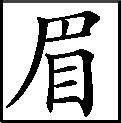
\includegraphics[width=3mm]{../Images/00010}\footnotesize \kaishu 一节颇似说辞,在{[}玉{]}兄口中却是衷肠之语。己卯冬夜。}说着不觉滴下泪来。{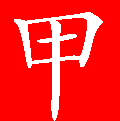
\includegraphics[width=3mm]{../Images/00002}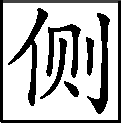
\includegraphics[width=3mm]{../Images/00011}\footnotesize \kaishu 玉兄泪非容易有的。}

黛玉耳内听了这话,眼内见了这形景,心内不觉灰了大半,也不觉滴下泪来,低头不语。宝玉见他这般形景,遂又说道:``我也知道我如今不好了,但只凭着怎么不好,万不敢在妹妹跟前有错处。{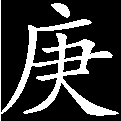
\includegraphics[width=3mm]{../Images/00004}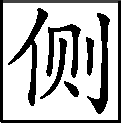
\includegraphics[width=3mm]{../Images/00011}\footnotesize \kaishu 有是语。}便有一二分错处,你倒是或教导我,戒我下次,{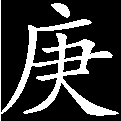
\includegraphics[width=3mm]{../Images/00004}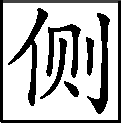
\includegraphics[width=3mm]{../Images/00011}\footnotesize \kaishu 可怜语。}或骂我两句,打我两下,我都不灰心。谁知你总不理我,{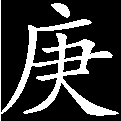
\includegraphics[width=3mm]{../Images/00004}\includegraphics[width=3mm]{../Images/00011}\footnotesize \kaishu 实难为情。}叫我摸不着头脑,少魂失魄,不知怎么样才是。{\includegraphics[width=3mm]{../Images/00004}\includegraphics[width=3mm]{../Images/00011}\footnotesize \kaishu 真有是事。}就便死了,也是个屈死鬼,任凭高僧高道忏悔也不能超升,{\includegraphics[width=3mm]{../Images/00004}\includegraphics[width=3mm]{../Images/00011}\footnotesize \kaishu 又瞒看官及批书人。}还得你申明了缘故,我才得托生呢!''

黛玉听了这个话,不觉将昨晚的事都忘在九霄云外了,{\includegraphics[width=3mm]{../Images/00002}\includegraphics[width=3mm]{../Images/00011}\footnotesize \kaishu ``情情''本来面目也。 \includegraphics[width=3mm]{../Images/00004}\includegraphics[width=3mm]{../Images/00011}\footnotesize \kaishu ``情情''衷肠。}便说道:``你既这么说,昨儿为什么我去了,你不叫丫头开门?''{\includegraphics[width=3mm]{../Images/00004}\includegraphics[width=3mm]{../Images/00011}\footnotesize \kaishu 正文,该问。}宝玉诧异道:``这话从那里说起?{\includegraphics[width=3mm]{../Images/00004}\includegraphics[width=3mm]{../Images/00011}\footnotesize \kaishu 实实不知。}我要是这么样,立刻就死了!''{\includegraphics[width=3mm]{../Images/00002}\includegraphics[width=3mm]{../Images/00011}\footnotesize \kaishu 急了。}林黛玉啐道:{\includegraphics[width=3mm]{../Images/00004}\includegraphics[width=3mm]{../Images/00011}\footnotesize \kaishu 如闻。}``大清早死呀活的,也不忌讳。你说有呢就有,没有就没有,起什么誓呢。''宝玉道:``实在没有见你去。就是宝姐姐坐了一坐,{\includegraphics[width=3mm]{../Images/00004}\includegraphics[width=3mm]{../Images/00011}\footnotesize \kaishu 不用兄言,彼已亲睹。}就出来了。''林黛玉想了一想,笑道:``想必是你的丫头们懒怠动,丧声歪气的也是有的。''宝玉道:``想必是这个原故。等我回去问了是谁,教训教训他们就好了。''{\includegraphics[width=3mm]{../Images/00004}\includegraphics[width=3mm]{../Images/00011}\footnotesize \kaishu 玉兄口气毕真。}黛玉道:``你的那些姑娘们{\includegraphics[width=3mm]{../Images/00004}\includegraphics[width=3mm]{../Images/00011}\footnotesize \kaishu 不快活之称。}也该教训教训,{\includegraphics[width=3mm]{../Images/00004}\includegraphics[width=3mm]{../Images/00011}\footnotesize \kaishu 照样的妙!}只是论理我不该说。今儿得罪了我的事小,倘或明儿宝姑娘来,什么贝姑娘来,{\includegraphics[width=3mm]{../Images/00004}\includegraphics[width=3mm]{../Images/00011}\footnotesize \kaishu 也还一句,的是心坎上人。}也得罪了,事情岂不大了。''说着抿着嘴笑。{\includegraphics[width=3mm]{../Images/00002}\includegraphics[width=3mm]{../Images/00011}\footnotesize \kaishu 至此心事全无矣。}宝玉听了,又是咬牙,又是笑。

二人正说话,只见丫头来请吃饭,{\includegraphics[width=3mm]{../Images/00002}\includegraphics[width=3mm]{../Images/00011}\footnotesize \kaishu 收拾得干净。}遂都往前头来了。王夫人见了林黛玉,因问道:``大姑娘,你吃那鲍太医的药可好些?''{\includegraphics[width=3mm]{../Images/00004}\includegraphics[width=3mm]{../Images/00011}\footnotesize \kaishu 是新换了的口气。}林黛玉道:``也不过这么着。老太太还叫我吃王大夫的药呢。''{\includegraphics[width=3mm]{../Images/00004}\includegraphics[width=3mm]{../Images/00011}\footnotesize \kaishu 何如?}宝玉道:``太太不知道,林妹妹是内症,先天生的弱,所以禁不住一点风寒,不过吃两剂煎药,疏散了风寒,还是吃丸药{\includegraphics[width=3mm]{../Images/00002}\includegraphics[width=3mm]{../Images/00011}\footnotesize \kaishu 引下文。}的好。''王夫人道:``前儿大夫说了个丸药的名字,我也忘了。''宝玉道:``我知道那些丸药,不过叫他吃什么人参养荣丸。''王夫人道:``不是。''宝玉又道:``八珍益母丸?左归?右归?再不,就是麦味地黄丸。''王夫人道:``都不是。我只记得有个`金刚'两个字的。''{\includegraphics[width=3mm]{../Images/00002}\includegraphics[width=3mm]{../Images/00011}\footnotesize \kaishu 奇文奇语。}宝玉扎手笑道:{\includegraphics[width=3mm]{../Images/00002}\includegraphics[width=3mm]{../Images/00011}\footnotesize \kaishu 慈母前放肆了。}``从来也没听见有个什么`金刚丸'。若有了`金刚丸',自然有`菩萨散'了!''{\includegraphics[width=3mm]{../Images/00002}\includegraphics[width=3mm]{../Images/00011}\footnotesize \kaishu 宝玉因黛玉事完,一心无挂碍,故不知不觉手之舞之,足之蹈之。 \includegraphics[width=3mm]{../Images/00004}\includegraphics[width=3mm]{../Images/00010}\footnotesize \kaishu 此写玉兄,亦是释却心中一夜半日要事,故大大一泄。己卯冬夜。}说的满屋里人都笑了。宝钗笑道:``想是天王补心丹。''{\includegraphics[width=3mm]{../Images/00002}\includegraphics[width=3mm]{../Images/00011}\footnotesize \kaishu 慧心人自应知之。}王夫人笑道:``是这个名儿。如今我也糊涂了。''宝玉道:``太太倒不糊涂,都是叫`金刚'`菩萨'支使糊涂了。''{\includegraphics[width=3mm]{../Images/00002}\includegraphics[width=3mm]{../Images/00011}\footnotesize \kaishu 是语甚对,余幼时所闻之语合符,哀哉伤哉!}王夫人道:``扯你娘的臊!又欠你老子捶你了。''{\includegraphics[width=3mm]{../Images/00004}\includegraphics[width=3mm]{../Images/00011}\footnotesize \kaishu 伏线。}宝玉笑道:``我老子再不为这个捶我的。''{\includegraphics[width=3mm]{../Images/00002}\includegraphics[width=3mm]{../Images/00011}\footnotesize \kaishu 此语亦不假。}

王夫人又道:``既有这个名儿,明日就叫人买些来。''{\includegraphics[width=3mm]{../Images/00004}\includegraphics[width=3mm]{../Images/00010}\footnotesize \kaishu 写药案是暗度颦卿病势渐加之笔,非泛泛闲文也。丁亥夏。畸笏叟。}宝玉道:``这些药都是不中用的。太太给我三百六十两银子,我给妹妹配一料丸药,包管一料不完就好了。''王夫人道:``放屁!什么药就这么贵?''宝玉道:``当真的呢,我这方子比别个不同。这个药名儿也古怪,一时也说不清。只讲那头胎紫河车,{\includegraphics[width=3mm]{../Images/00004}\includegraphics[width=3mm]{../Images/00011}\footnotesize \kaishu 只闻名。}人形带叶参,三百六十两不足。\href{../Text/part0032_split_000.html\#lnkback_2_a}{\textsuperscript{②}}龟大何首乌,{\includegraphics[width=3mm]{../Images/00004}\includegraphics[width=3mm]{../Images/00011}\footnotesize \kaishu 听也不曾听过。}千年松根茯苓胆,{\includegraphics[width=3mm]{../Images/00004}\includegraphics[width=3mm]{../Images/00010}\footnotesize \kaishu 写得不犯冷香丸方子。◇前``玉生香''回中,颦云``他有金你有玉;他有冷香你岂不该有暖香?''是宝玉无药可配矣。今颦儿之剂,若许材料皆系滋补热性之药,兼有许多奇物,而尚未拟名,何不竟以``暖香''名之?以代补宝玉之不足,岂不三人一体矣。己卯冬夜。}诸如此类的药都不算为奇,{\includegraphics[width=3mm]{../Images/00004}\includegraphics[width=3mm]{../Images/00011}\footnotesize \kaishu 还有奇的。}只在群药里算。那为君的药,说起来唬人一跳。前儿薛大哥求了我有一二年,我才给了他这个方子。他拿了方子去又寻了二三年,花了有上千的银子,才配成了。太太不信,只问宝姐姐。''宝钗听说,笑着摇手儿道:``我不知道,也没听见。你别叫姨娘问我。''王夫人笑道:``到底是宝丫头,好孩子,不撒谎。''宝玉站在当地,听见如此说,一回身把手一拍,说道:``我说的倒是真话呢,倒说我撒谎。''说着一回身,只见黛玉坐在宝钗身后抿着嘴笑,用手指在脸上画着羞他。{\includegraphics[width=3mm]{../Images/00004}\includegraphics[width=3mm]{../Images/00011}\footnotesize \kaishu 好看煞,在颦儿必有之。}

凤姐因在里间屋里看着人放桌子,{\includegraphics[width=3mm]{../Images/00004}\includegraphics[width=3mm]{../Images/00011}\footnotesize \kaishu 且不接宝玉文字,妙!}听如此说,便走来笑道:``宝兄弟不是撒谎,这倒是有的。上月薛大哥亲自和我寻珍珠,我问他作什么,他说是配药。他还抱怨说,不配也罢了,如今那里知道这么费事。我问他什么药,他说是宝兄弟的方子,说了多少药,我也没工夫听。他说:`不然我也买几颗珍珠了,只是定要头上戴过的,所以来和你寻。'他说:`妹妹若没散的,花儿上也得,掐下来,过后儿我拣好的再给妹妹穿了来。'我没法儿,把两枝珠花现拆了给他。还要了一块三尺大红库纱去,乳钵乳了隔面子呢。''凤姐说一句,宝玉念一句佛,说:``太阳在屋里呢!''凤姐说完了,宝玉又道:``太太想,这不过是将就呢。正经按那方子,这珍珠宝石定要古坟里的,有那古时富贵人家装裹的头面,拿了来才好。如今那里为这个去刨坟掘墓,所以只要活人戴过的,也可以使得。''王夫人随念:``阿弥陀佛,不当家花花的!就是坟里有这个,人家死了几百年,如今翻尸盗骨的,作了药也不灵!''{\includegraphics[width=3mm]{../Images/00002}\includegraphics[width=3mm]{../Images/00011}\footnotesize \kaishu 不止阿凤圆谎,今作者亦为圆谎了,看此数句则知矣。}

宝玉向林黛玉说道:``你听见了没有,难道二姐姐也跟着我撒谎不成?''脸望着黛玉说话,却拿眼睛飘着宝钗。黛玉便拉王夫人道:``舅母听听,宝姐姐不替他圆谎,他直问着我。''王夫人也道:``宝玉很会欺负你妹妹。''宝玉笑道:``太太不知道原故。宝姐姐先在家里住着,那薛大哥的事,他就不知道,何况如今在里头住着呢,自然是越发不知道了。{\includegraphics[width=3mm]{../Images/00004}\includegraphics[width=3mm]{../Images/00011}\footnotesize \kaishu 分析的是,不敢正犯。}林妹妹才在背后,以为是我撒谎,就羞我。''

说着,只见贾母房里的丫头找宝玉、黛玉吃饭。林黛玉也不叫宝玉,便起身拉了那丫头就走。那丫头说等着宝玉一块儿走。林黛玉道:``他不吃饭了,咱们走吧。\href{../Text/part0032_split_000.html\#lnkback_3_a}{\textsuperscript{③}}我先走了。''说着便出去了。宝玉道:``我今儿还跟着太太吃罢。''王夫人道:``罢,罢,我今儿吃斋,你正经吃去罢。''宝玉道:``我也跟着吃斋。''说着便叫那丫头``去罢'',自己先跑到炕上坐了。王夫人向宝钗道:``你们只管吃你们的去,由他罢。''宝钗因笑道:``你正经去罢。吃不吃,陪着林妹妹走一趟,他心里打紧的不自在呢。''宝玉道:``理他呢,过一会子就好了。''{\includegraphics[width=3mm]{../Images/00004}\includegraphics[width=3mm]{../Images/00011}\footnotesize \kaishu 后文方知。}

一时吃过饭,宝玉一则怕贾母记挂,二则也记挂着黛玉,忙忙的要茶漱口。探春、惜春都笑道:``二哥哥,你成日家忙些什么?{\includegraphics[width=3mm]{../Images/00002}\includegraphics[width=3mm]{../Images/00011}\footnotesize \kaishu 冷眼人自然了了。}吃饭吃茶也是这么忙碌碌的。''宝钗笑道:``你叫他快吃了瞧林妹妹去罢,叫他在这里胡羼些什么。''宝玉吃了茶便出来,直往西院走。可巧走到凤姐院前,只见凤姐蹬着门槛子拿耳挖子剔牙,{\includegraphics[width=3mm]{../Images/00004}\includegraphics[width=3mm]{../Images/00011}\footnotesize \kaishu 也才吃了饭。}看着小子们挪花盆呢。{\includegraphics[width=3mm]{../Images/00004}\includegraphics[width=3mm]{../Images/00011}\footnotesize \kaishu 是阿凤身段。}见宝玉来了,笑道:``你来的正好。进来,进来,{\includegraphics[width=3mm]{../Images/00004}\includegraphics[width=3mm]{../Images/00011}\footnotesize \kaishu 如闻。}替我写几个字儿。''宝玉只得跟了进来。到了房里,凤姐命人取过笔砚纸来,向宝玉道:``大红妆缎四十匹,蟒缎四十匹,上用纱各色一百匹,金项圈四个。''宝玉道:``这算什么?又不是账,又不是礼物,怎么个写法?''凤姐道:``你只管写上,横竖我自己明白就罢了。''{\includegraphics[width=3mm]{../Images/00004}\includegraphics[width=3mm]{../Images/00011}\footnotesize \kaishu 有是语,有是事。}宝玉听说,只得写了。凤姐收起来,笑道:``还有句话告诉你,不知你依不依?你屋里有个丫头叫红玉,我和你说说,要叫了来使唤,也总没得说,今儿见你才想起来。''{\includegraphics[width=3mm]{../Images/00002}\includegraphics[width=3mm]{../Images/00011}\footnotesize \kaishu 字眼。}宝玉道:``我屋里的人也多的很,姐姐喜欢谁,只管叫了来,何必问我。''{\includegraphics[width=3mm]{../Images/00002}\includegraphics[width=3mm]{../Images/00011}\footnotesize \kaishu 红玉接杯倒茶,自纱屉内觅至回廊下,再见此处如此写来,可知玉兄除颦儿外,俱是行云流水。}凤姐笑道:``既这么着,我就叫人带他去了。''{\includegraphics[width=3mm]{../Images/00002}\includegraphics[width=3mm]{../Images/00011}\footnotesize \kaishu 又了却怡红一冤孽,一叹!}宝玉道:``只管带去。''说着便要走。{\includegraphics[width=3mm]{../Images/00002}\includegraphics[width=3mm]{../Images/00011}\footnotesize \kaishu 忙极!}凤姐道:``你回来,我还有句话说。''宝玉道:``老太太叫我呢,{\includegraphics[width=3mm]{../Images/00002}\includegraphics[width=3mm]{../Images/00011}\footnotesize \kaishu 非也,林妹妹叫我呢。一笑。}有话等我回来罢。''说着,便来至贾母这边,已经都吃完了饭。贾母因问他:``跟着你母亲吃什么好的了?''宝玉笑道:``也没什么好的,我倒多吃了一碗饭。''{\includegraphics[width=3mm]{../Images/00002}\includegraphics[width=3mm]{../Images/00011}\footnotesize \kaishu 安慰祖母之心也。}因问:``林妹妹在那里呢?''{\includegraphics[width=3mm]{../Images/00002}\includegraphics[width=3mm]{../Images/00011}\footnotesize \kaishu 何如?余言不谬。}贾母道:``里头屋里呢。''

宝玉进来,只见地下一个丫头吹熨斗,炕上两个丫头打粉线,黛玉弯着腰,拿着剪子裁什么呢。宝玉走进来笑道:``哦,{\includegraphics[width=3mm]{../Images/00004}\includegraphics[width=3mm]{../Images/00011}\footnotesize \kaishu 句。}这是作什么呢?才吃了饭,这么空着头,一会子又头疼了。''黛玉并不理,只管裁他的。有一个丫头道:``这块绸子角儿还不好呢,再熨他一熨。''黛玉把剪子一撂,说道:``理他呢,过一会子就好了。''{\includegraphics[width=3mm]{../Images/00002}\includegraphics[width=3mm]{../Images/00011}\footnotesize \kaishu 有意无意,暗合针对,无怪{[}玉兄纳闷{]}。}宝玉听了,只是纳闷。只见宝钗、探春也来了,和贾母说了一会话。宝钗也进来问:``林妹妹作什么呢?''见黛玉裁剪,因笑道:``越发能干了,连裁剪都会了。''黛玉笑道:``这也不过是撒谎哄人罢了。''宝钗笑道:``我告诉你个笑话儿,才刚为那个药,我说了个不知道,宝玉心里不受用了。''林黛玉道:``理他呢,过一会子就好了。''{\includegraphics[width=3mm]{../Images/00002}\includegraphics[width=3mm]{../Images/00010}\footnotesize \kaishu 连重二次前言,是颦、宝气味暗合,勿认作有小人过言也。 \includegraphics[width=3mm]{../Images/00004}\includegraphics[width=3mm]{../Images/00010}\footnotesize \kaishu 连重两遍前言,是颦、玉气味相仿,无非偶然暗合相符,勿认作有过言小人也。}宝玉又向宝钗道:``老太太要抹骨牌,正没人,你抹骨牌去。''宝钗听说,便笑道:``我是为抹骨牌才来了?''说着便走了。林黛玉道:``你倒是去罢,这里有老虎,看吃了你!''说着又裁。宝玉见他不理,只得还陪笑说道:``你也去逛逛再裁不迟。''黛玉总不理。宝玉便问丫头们:``这是谁叫裁的?''黛玉见问丫头们,便说道:``凭他谁叫裁,不管二爷的事!''宝玉听了,方欲说话,只见有人进来回说``外头有人请你呢''。宝玉听说,忙撤身出来。黛玉向外说道:{\includegraphics[width=3mm]{../Images/00002}\includegraphics[width=3mm]{../Images/00011}\footnotesize \kaishu 仍丢不下,叹叹!}``阿弥陀佛!赶你回来,我死了也罢了。''{\includegraphics[width=3mm]{../Images/00002}\includegraphics[width=3mm]{../Images/00011}\footnotesize \kaishu 何苦来?余不忍听。}

宝玉出来,到外头,只见茗烟说道:``冯大爷家请。''宝玉听了,知道是昨日的话,便说:``要衣裳去。''自己便往书房里来。茗烟一直到了二门前等人,{\includegraphics[width=3mm]{../Images/00002}\includegraphics[width=3mm]{../Images/00011}\footnotesize \kaishu 此门请出玉兄来,故信步又至书房,文人弄墨,虚点缀也。}只见出来个老婆子,茗烟上去说道:``宝二爷在书房里等出门的衣裳,你老人家进去带个信儿。''那婆子说:``你妈的屄!{\includegraphics[width=3mm]{../Images/00004}\includegraphics[width=3mm]{../Images/00011}\footnotesize \kaishu 活现活跳。}倒好,宝二爷如今在园子里住着,{\includegraphics[width=3mm]{../Images/00002}\includegraphics[width=3mm]{../Images/00011}\footnotesize \kaishu 与夜间叫人对看。}跟他的人都在园子里,你又跑了这里来带信儿!''茗烟听了,笑道:``骂的是,我也糊涂了。''说着一径往东边二门上来。可巧门上小厮在甬路底下踢球,茗烟将原故说了。有个小厮跑了进去,半日才抱了一个包袱出来,递与茗烟。回到书房里,宝玉换了,命人备马,只带着茗烟、锄药、双瑞、双寿四个小厮,一径来到冯紫英门口。有人报与冯紫英,出来迎接进去。只见薛蟠早已在那里久候,还有许多唱曲儿的小厮并唱小旦的蒋玉菡、锦香院的妓女云儿。大家都见过了,然后吃茶。

宝玉擎茶笑道:``前儿所言幸与不幸之事,我昼悬夜想,今日一闻呼唤即至。''冯紫英笑道:``你们令表兄弟倒都心实。前日不过是我的设辞,诚心请你们一饮,恐又推托,故说下这句话。{\includegraphics[width=3mm]{../Images/00002}\includegraphics[width=3mm]{../Images/00010}\footnotesize \kaishu 若真有一事,则不成《石头记》文字矣。作者得三昧在兹,批书人得书中三昧亦在兹。{[}壬午孟夏。{]}}今日一邀即至,谁知都信真了。''说毕大家一笑,然后摆上酒来,依次坐定。冯紫英先命唱曲儿的小厮过来让酒,然后命云儿也来敬。

那薛蟠三杯下肚,不觉忘了情,拉着云儿的手笑道:``你把那梯己新样儿的曲子唱个我听,我吃一坛如何?''云儿听说,只得拿起琵琶来,唱道:

两个冤家,都难丢下,想着你来又记挂着他。两个人形容俊俏,都难描画。想昨宵幽期私订在荼蘼架,一个偷情,一个寻拿,拿住了三曹对案,我也无回话。{\includegraphics[width=3mm]{../Images/00002}\includegraphics[width=3mm]{../Images/00011}\footnotesize \kaishu 此唱一曲为直刺宝玉。}

唱毕笑道:``你喝一坛子罢了。''薛蟠听说,笑道:``不值一坛,再唱好的来。''

宝玉笑道:``听我说来:如此滥饮,易醉而无味。我先吃一大海,{\includegraphics[width=3mm]{../Images/00004}\includegraphics[width=3mm]{../Images/00010}\footnotesize \kaishu 大海饮酒,西堂产九台灵芝日也,批书至此,宁不悲乎?壬午重阳日。}发一新令,有不遵者,连罚十大海,逐出席外与人斟酒。''{\includegraphics[width=3mm]{../Images/00002}\includegraphics[width=3mm]{../Images/00011}\footnotesize \kaishu 谁曾经过?叹叹!西堂故事。}冯紫英、蒋玉菡等都道:``有理,有理。''宝玉拿起海来,一气饮尽,说道:``如今要说悲、愁、喜、乐四字,都要说出女儿来,还要注明这四字的原故。说完了,饮门杯。酒面要唱一个新鲜时样的曲子;酒底要席上生风一样东西,或古诗旧对、《四书》《五经》成语。''薛蟠未等说完,先站起来拦住道:``我不来,别算我。{\includegraphics[width=3mm]{../Images/00002}\includegraphics[width=3mm]{../Images/00011}\footnotesize \kaishu 爽人爽语。}这竟是捉弄我呢!''{\includegraphics[width=3mm]{../Images/00004}\includegraphics[width=3mm]{../Images/00011}\footnotesize \kaishu 岂敢?}云儿便站起来,推他坐下,笑道:``怕什么?这还亏你天天吃酒呢,难道连我也不如!我回来还说呢。说是了,罢;不是了,不过罚上几杯,那里就醉死了。你如今一乱令,倒喝十大杯,下去给人斟酒不成?''{\includegraphics[width=3mm]{../Images/00004}\includegraphics[width=3mm]{../Images/00011}\footnotesize \kaishu 有理。}众人都拍手道妙。薛蟠听说,无法可治,只得坐下。听宝玉先说,宝玉便道:

女儿悲,青春已大守空闺。

女儿愁,悔教夫婿觅封侯。

女儿喜,对镜晨妆颜色美。

女儿乐,秋千架上春衫薄。

众人听了,都道:``说得有理。''薛蟠独扬着脸摇头说:``不好,该罚!''众人问:``如何该罚?''薛蟠道:``他说的我都不懂,怎么不该罚?''云儿便拧他一把,笑道:``你悄悄的想你的罢。回来说不出,才是该罚呢。''于是拿琵琶听宝玉唱道:

滴不尽相思血泪抛红豆,开不完春柳春花满画楼。睡不稳纱窗风雨黄昏后,忘不了新愁与旧愁,咽不下玉粒金莼噎满喉,照不见菱花镜里形容瘦。展不开的眉头,捱不明的更漏。呀!恰便似遮不住的青山隐隐,流不断的绿水悠悠。

唱完,大家齐声喝彩,独薛蟠说无板。宝玉饮了门杯,便拈起一片梨来,说道:``雨打梨花深闭门。''完了令。

下该冯紫英。听冯紫英说道:

女儿悲,儿夫染病在垂危。

女儿愁,大风吹倒梳妆楼。

女儿喜,头胎养了双生子。

女儿乐,私向花园掏蟋蟀。{\includegraphics[width=3mm]{../Images/00002}\includegraphics[width=3mm]{../Images/00012}\footnotesize \kaishu 紫英口中应当如是。}

说毕,端起酒来,唱道:

你是个可人,你是个多情,你是个刁钻古怪鬼灵精,你是个神仙也不灵。我说的话儿你全不信,只叫你去背地里细打听,才知道我疼你不疼!

唱完,饮了门杯,说道:``鸡鸣茅店月。''令完,下该云儿。云儿便说道:

女儿悲,将来终身指靠谁?{\includegraphics[width=3mm]{../Images/00002}\includegraphics[width=3mm]{../Images/00012}\footnotesize \kaishu 道着了。}

薛蟠叹道:``我的儿,有你薛大爷在,你怕什么!''众人都道:``别混他,别混他!''云儿又道:

女儿愁,妈妈打骂何时休!

薛蟠道:``前儿我见了你妈,还吩咐他不叫他打你呢。''众人都道:``再多言者罚酒十杯。''薛蟠连忙自己打了一个嘴巴子,说道:``没耳性,再不许说了。''云儿又道:

女儿喜,情郎不舍还家里。

女儿乐,住了箫管弄弦索。

说完,便唱道:

豆蔻开花三月三,一个虫儿往里钻。钻了半日不得进去,爬到花儿上打秋千。肉儿小心肝,我不开了你怎么钻?{\includegraphics[width=3mm]{../Images/00002}\includegraphics[width=3mm]{../Images/00012}\footnotesize \kaishu 双关,妙!}

唱毕,饮了门杯,说道:``桃之夭夭。''令完了,下该薛蟠。

薛蟠道:``我可要说了:女儿悲------''说了半日,不见说底下的。冯紫英笑道:``悲什么?快说来。''薛蟠登时急的眼睛铃铛一般,瞪了半日,才说道:``女儿悲------''又咳嗽了两声,{\includegraphics[width=3mm]{../Images/00002}\includegraphics[width=3mm]{../Images/00011}\footnotesize \kaishu 受过此急者,大都不止呆兄一人耳。}说道:``女儿悲,嫁了个男人是乌龟。''众人听了都大笑起来。{\includegraphics[width=3mm]{../Images/00002}\includegraphics[width=3mm]{../Images/00010}\footnotesize \kaishu 此段与《金瓶梅》内西门庆、应伯爵在李桂姐家饮酒一回对看,未知孰家生动活泼?}薛蟠道:``笑什么,难道我说的不是?一个女儿嫁了汉子,要当忘八,他怎么不伤心呢?''众人笑的弯腰,说道:``你说的很是,快说底下的。''薛蟠瞪了瞪眼,又说道:``女儿愁------''说了这句,又不言语了。众人道:``怎么愁?''薛蟠道:``女儿愁,绣房撺出个大马猴。''{\includegraphics[width=3mm]{../Images/00002}\includegraphics[width=3mm]{../Images/00011}\footnotesize \kaishu 不愁,一笑。}众人呵呵笑道:``该罚,该罚!这句更不通,先还可恕。''说着便要筛酒。宝玉笑道:``押韵就好。''薛蟠道:``令官都准了,你们闹什么?''众人听说,方罢了。云儿笑道:``下两句越发难说了,我替你说罢。''薛蟠道:``胡说!当真的我就没好的了!听我说罢:女儿喜,洞房花烛朝慵起。''众人听了,都诧异道:``这句何其太韵?''薛蟠又道:``女儿乐,一根\includegraphics[width=8mm]{../images/00022}往里戳。''{\includegraphics[width=3mm]{../Images/00002}\includegraphics[width=3mm]{../Images/00011}\footnotesize \kaishu 有前韵句,故有是句。}众人听了,都扭着脸说道:``该死,该死!快唱了罢。''薛蟠便唱道:``一个蚊子哼哼哼。''众人都怔了,说``这是个什么曲儿?''薛蟠还唱道:``两个苍蝇嗡嗡嗡。''众人都道:``罢,罢,罢!''薛蟠道:``爱听不听!这个新鲜曲儿,叫作哼哼韵。你们要懒待听,连酒底都免了,我就不唱。''{\includegraphics[width=3mm]{../Images/00002}\includegraphics[width=3mm]{../Images/00011}\footnotesize \kaishu 何尝呆?}众人都道:``免了罢,倒别耽误了别人家。''于是蒋玉菡说道:

女儿悲,丈夫一去不回归。

女儿愁,无钱去打桂花油。

女儿喜,灯花并头结双蕊。{\includegraphics[width=3mm]{../Images/00002}\includegraphics[width=3mm]{../Images/00011}\footnotesize \kaishu 佳谶也。}

女儿乐,夫唱妇随真和合。

说毕,唱道:

可喜你天生成百媚娇,恰便似活神仙离云霄。度青春,年正小;配鸾凤,真也着。呀!看天河正高,听谯楼鼓敲,剔银灯同入鸳帏悄。

唱毕,饮了门杯,笑道:``这诗词上我倒有限。幸而昨日见了一副对子,可巧{\includegraphics[width=3mm]{../Images/00002}\includegraphics[width=3mm]{../Images/00011}\footnotesize \kaishu 真巧!}只记得这句,幸而席上还有这件东西。''{\includegraphics[width=3mm]{../Images/00002}\includegraphics[width=3mm]{../Images/00011}\footnotesize \kaishu 瞒过众人。}说毕,便饮干了酒,拿起一朵木樨来,念道:``花气袭人知昼暖。''

众人倒都依了,完令。薛蟠又跳了起来,喧嚷道:``了不得,了不得!该罚,该罚!这席上并没有宝贝,{\includegraphics[width=3mm]{../Images/00002}\includegraphics[width=3mm]{../Images/00011}\footnotesize \kaishu 奇谈。}你怎么念起宝贝来?''蒋玉菡怔了,说道:``何曾有宝贝?''薛蟠道:``你还赖呢!你再念来。''蒋玉菡只得又念了一遍。薛蟠道:``袭人可不是宝贝是什么!你们不信,只问他。''说着,指着宝玉。宝玉没好意思起来,说道:``薛大哥,你该罚多少?''薛蟠道:``该罚,该罚!''说着拿起酒来,一饮而尽。冯紫英与蒋玉菡等不知原故,犹问原故,云儿便告诉了出来。{\includegraphics[width=3mm]{../Images/00002}\includegraphics[width=3mm]{../Images/00011}\footnotesize \kaishu 用云儿细说,的是章法。 \includegraphics[width=3mm]{../Images/00004}\includegraphics[width=3mm]{../Images/00010}\footnotesize \kaishu 云儿知怡红细事,可想玉兄之风情意也。壬午重阳。}蒋玉菡忙起身陪罪。众人都道:``不知者不作罪。''

少刻,宝玉席外解手,蒋玉菡便随了出来。二人站在廊檐底下,蒋玉菡又陪不是。宝玉见他妩媚温柔,心中十分留恋,便紧紧的搭着他的手,叫他:``闲了往我们这里来。还有一句话借问,也是你们贵班中,有一个叫琪官的,他在那里?如今名驰天下,我独无缘一见。''蒋玉菡笑道:``就是我的小名儿。''宝玉听说,不觉欣然跌足笑道:``有幸,有幸!果然名不虚传。今儿初会,便怎么样呢?''想了一想,向袖中取出扇子,将一个玉玦扇坠解下来,递与琪官道:``微物不堪,略表初见之谊。''琪官接了,笑道:``无功受禄,何以克当!也罢,我这里也得了一件奇物,今日早起方系上,还是簇新的,聊可表我一点亲热之意。''说着,将系小衣儿一条大红汗巾子解下来,递与宝玉,道:``这汗巾是茜香国女国王进贡来的,夏天系着,肌肤生香,不生汗渍。昨日北静王给我的,今日才上身。若是别人,我断不肯相赠。二爷请把自己系的给我系着。''宝玉听说,喜不自禁,连忙接了,将自己一条松花汗巾解了下来,递与琪官。{\includegraphics[width=3mm]{../Images/00002}\includegraphics[width=3mm]{../Images/00011}\footnotesize \kaishu 红绿{(牵)}{[}汗{]}巾是这样用法。一笑。}二人方束好,只听一声大叫:``我可拿住了!''只见薛蟠跳了出来,拉着二人道:``放着酒不吃,两个人逃席出来干什么?快拿出来我瞧瞧。''二人都道:``没什么。''薛蟠那里肯依,还是冯紫英出来才解开了。于是复又归座饮酒,至晚方散。

宝玉回至园中,宽衣吃茶。袭人见扇子上的扇坠儿没了,{\includegraphics[width=3mm]{../Images/00004}\includegraphics[width=3mm]{../Images/00011}\footnotesize \kaishu 身上事。}便问他:``往那里去了?''宝玉道:``马上丢了。''{\includegraphics[width=3mm]{../Images/00004}\includegraphics[width=3mm]{../Images/00011}\footnotesize \kaishu 随口谎言。}睡觉时只见腰里一条血点似的大红汗巾子,袭人便猜了八九分,因说道:``你有了好的系裤子,把我那条还我罢。''宝玉听说,方想起那条汗巾子原是袭人的,不该给人才是,心里后悔,口里说不出来,只得笑道:``我赔你一条罢。''袭人听了,点头叹道:``我就知道又干这些事!也不该拿着我的东西给那起混帐人去。也难为你心里没个算计儿。''再要说上几句,又恐怕怄上他的酒来,少不得睡了,一宿无话。

至次日天明起来,只见宝玉笑道:``夜里失了盗也不晓得,你瞧瞧裤子上。''袭人低头一看,只见昨日宝玉系的那条汗巾子系在自己腰里,便知是宝玉夜间换了,忙一顿把\href{../Text/part0032_split_000.html\#lnkback_4_a}{\textsuperscript{④}}解下來,说道:``我不希罕这行子,趁早儿拿了去!''宝玉见他如此,只得委婉解劝了一回。袭人无法,只得系上。过后宝玉出去,终久解下来,掷在个空箱子里,自己又换了一条系着。

宝玉并不理论,因问起昨日可有什么事情。袭人便回说道:``二奶奶打发了人叫了红玉去了。他原要等你来,我想什么要紧,我就作了主,打发他去了。''宝玉道:``很是。我已知道了,不必等我罢了。''袭人又道:``昨儿贵妃差了夏太监出来,送了一百二十两银子,叫在清虚观初一到初三打三天平安醮,唱戏献供,叫珍大爷领着众位爷们等跪香拜佛呢。还有端午儿的节礼也赏了。''说着命小丫头来,将昨日的所赐之物取了出来,只见上等宫扇两柄,红麝香珠二串,凤尾罗二端,芙蓉簟一领。宝玉见了,喜不自胜,问道:``别人的也都是这个么?''袭人道:``老太太的多着一个香如意,一个玛瑙枕。老爷、太太、姨太太的只多着一柄如意。你的同宝姑娘的一样。{\includegraphics[width=3mm]{../Images/00002}\includegraphics[width=3mm]{../Images/00011}\footnotesize \kaishu 金娃玉郎是这样写法。}林姑娘同二姑娘、三姑娘、四姑娘只单有扇子同数珠儿,别人都没了。大奶奶、二奶奶他两个是每人两匹纱、两匹罗、两个香袋儿、两个锭子药。''宝玉听了,笑道:``这是怎么个原故?怎么林姑娘的倒不同我的一样,倒是宝姐姐的同我一样!别是传错了罢?''袭人道:``昨儿拿出来,都是一份一份的写着签子,怎么就错了!你的是在老太太屋里来着,我去拿了来了。老太太说,明儿叫你一个五更天进去谢恩呢。''宝玉道:``自然要走一趟。''说着便叫紫绡:``来,拿了这个到林姑娘那里去,就说是昨儿我得的,爱什么留下什么。''紫绡答应了,便拿了去,不一时回来说:``林姑娘说了,昨儿也得了,二爷留着罢。''

宝玉听说,便命人收了。刚洗了脸出来,要往贾母那边请安去,只见林黛玉顶头来了。宝玉赶上去,笑道:``我的东西叫你拣,你怎么不拣?''林黛玉昨日所恼宝玉的心事早又丢开,只顾今日的事了,因说道:``我没这么大福禁受,比不得宝姑娘,什么金什么玉的,我们不过是草木之人!''{\includegraphics[width=3mm]{../Images/00002}\includegraphics[width=3mm]{../Images/00011}\footnotesize \kaishu 自道本是绛珠草也。}宝玉听他提出``金玉''二字来,不觉心动疑猜,便说道:``除了别人说什么金什么玉,我心里要有这个想头,天诛地灭,万世不得人身!''林黛玉听他这话,便知他心里动了疑,忙又笑道:``好没意思,白白的说什么誓?管你什么金什么玉的呢!''宝玉道:``我心里的事也难对你们说,日后自然明白。除了老太太、老爷、太太这三个人,第四个就是妹妹了。要有第五个人,我就说个誓。''黛玉道:``你也不用说誓,我很知道你心里有`妹妹',但只是见了`姐姐',就把`妹妹'忘了。''宝玉道:``那是你多心,我再不的。''黛玉道:``昨儿宝丫头不替你圆谎,为什么问着我呢?那要是我,你又不知怎么样了。''

正说着,只见宝钗从那边来了,二人便走开了。宝钗分明看见,只装看不见,低着头过去了,到了王夫人那里,坐了一回,然后到了贾母这边,只见宝玉在这里呢。{\includegraphics[width=3mm]{../Images/00002}\includegraphics[width=3mm]{../Images/00011}\footnotesize \kaishu 宝钗往王夫人处去,故宝玉先在贾母处,一丝不乱。}宝钗因往日母亲对王夫人等曾提过``金锁是个和尚给的,等日后有玉的方可结为婚姻''等语,{\includegraphics[width=3mm]{../Images/00002}\includegraphics[width=3mm]{../Images/00011}\footnotesize \kaishu 此处表明,以后二宝文章,宜换眼看。}所以总远着宝玉。{\includegraphics[width=3mm]{../Images/00002}\includegraphics[width=3mm]{../Images/00010}\footnotesize \kaishu 峰峦全露,又用烟云截断,好文字。}昨日见了元春所赐的东西,独他与宝玉一样,心里越发没意思起来。幸亏宝玉被一个黛玉缠绵住了,心心念念只记挂着黛玉,并不理论这事。此刻忽见宝玉笑问道:``宝姐姐,我瞧瞧你的那红麝串子。''可巧宝钗左腕上笼着一串,见宝玉问他,少不得褪了下来。宝钗原生的肌肤丰泽,容易褪不下来。宝玉在旁边看着雪白一段酥臂,不觉动了羡慕之心,暗暗想道:``这个膀子要长在林妹妹身上,或者还得摸一摸,偏生长在他身上。''正是恨没福得摸,忽然想起``金玉''一事来,再看看宝钗形容,只见脸若银盆,眼似水杏,唇不点而红,眉不画而翠,{\includegraphics[width=3mm]{../Images/00002}\includegraphics[width=3mm]{../Images/00011}\footnotesize \kaishu 太白所谓``清水出芙蓉''。}比黛玉另具一种妩媚风流,不觉就呆了,{\includegraphics[width=3mm]{../Images/00002}\includegraphics[width=3mm]{../Images/00011}\footnotesize \kaishu 忘情,非呆也。}宝钗褪了串子来递与他也忘了接。宝钗见他怔了,自己倒不好意思的,丢下串子,回身才要走,只见黛玉蹬着门槛子,嘴里咬着手帕子笑呢。宝钗道:``你又禁不得风儿吹,怎么又站在那风口里呢?''黛玉笑道:``何曾不是在屋里呢。只因听见天上一声叫,出来瞧了一瞧,原来是个呆雁。''宝钗道:``呆雁在那里呢?我也瞧瞧。''黛玉道:``我才出来,他就`忒儿'一声飞了。''口里说着,将手里的帕子一甩,向宝玉脸上甩来。不防正打在眼上,``嗳哟''了一声。再看下回分明。

{\includegraphics[width=3mm]{../Images/00002}\kaishu 总评:茜香罗、红麝串写于一回,盖琪官虽系优人,后回与袭人供奉玉兄宝卿得同终始者,非泛泛之文也。}

{\kaishu 自``闻曲''回以后,回回写药方,是白描颦儿添病也。}

{\kaishu 前``玉生香''回中颦云``他有金你有玉;他有冷香你岂不该有暖香?''是宝玉无药可配矣。今颦儿之剂若许材料皆系滋补热性之药,兼有许多奇物,而尚未拟名,何不竟以``暖香''名之?以代补宝玉之不足,岂不三人一体矣。}

{\kaishu 宝玉忘情,露于宝钗,是后回累累忘情之引。}

{\kaishu 茜香罗暗系于袭人腰中,系伏线之文。}

{\includegraphics[width=3mm]{../Images/00005}\kaishu 总评:世间最苦是痴情,不遇知音休应声。盟誓已成了,莫迟误今生。}

%{\href{../Text/part0032_split_000.html\#navto_1_a}{①}庚辰本也有此批,内容基本相同,唯末句作``幸甚幸甚''。按此批与上回末的朱批应为同时所作,而且甲戌本(原本)显然是从庚辰本(原本)过录的。故末句应以``幸甚幸甚''为是。甲戌本致误原因是:传抄过程中某本误``幸''为``本''(此本已有第一回``是书何本''、第二十五回``看书人亦要如是看为本''两误例),后之转抄者以``本''字不通,据文意改为音同形近的``笨''字。}
%
%{\href{../Text/part0032_split_000.html\#navto_2_a}{②}``三百六十两不足'':此句列藏本缺,杨本为旁添,戚、蒙本``不足''作``还不够''。此语是宝玉对前文王夫人问``什么药就这么贵''的解释,也可能是批书人的批注。有人把``三百六十两''和``不足''断开分别归前后句,非是。}
%
%{\href{../Text/part0032_split_000.html\#navto_3_a}{③}列、杨本此处多29字,作``\,`(咱们走)吧。'那丫头道:`吃不吃,等他一块儿去。老太太问,让他说去。'黛玉道:`你就等着。(我先走了。)'\,''似觉语气更连贯自然。}
%
%{\href{../Text/part0032_split_000.html\#navto_4_a}{④}一顿把:北方方言。形容动作的快速,犹言``一下子''、``一古脑儿''。}
